\documentclass[12pt,abstracton,a4paper]{scrartcl}
\usepackage{lmodern}
\usepackage{graphicx}
\usepackage{epstopdf}
\usepackage{amsmath}
\usepackage{amsfonts}
\usepackage{algorithm}
\usepackage{algorithmic}
\usepackage{subfigure}
%\usepackage[sections=normal,title=normal]{savetrees}
\usepackage[colorlinks]{hyperref}
\usepackage[sorting=none]{biblatex}
\bibliography{bibliography}

% definitions
\def\eqd{\,{\buildrel d \over =}\,}
\def\x{{\bf x}}
\def\z{{\bf z}}
\def\figwidth{0.31\linewidth}

\title{Topic Models for Twitter User Profiling}
\author{
\begin{tabular}{cc}
    Jan Vosecky & Mathis Antony  \\
    \href{mailto:jvosecky@ust.hk}{jvosecky@ust.hk} &
    \href{mailto:mantony@ust.hk}{mantony@ust.hk}
\end{tabular}
\\ The Hong Kong University of Science and Technology 
\\ Clear Water Bay 
\\ Hong Kong} 
\begin{document}
\maketitle

\begin{abstract}
We propose, implement and analyze two new topic models for twitter user profiling. A challenging aspect of the problem is the evolution of the users and the topics of interests in the general population. We use stochastic variational inference allowing for scalability and treatment of streaming data. We analyze the perplexity of our models output and compare them with the well established Latent Dirichlet Allocation topic model.
\end{abstract}

\section{Introduction}
Latent Dirichlet Allocation (LDA) is a topic model originally invented by Blei et al. \cite{Blei03} as an unsupervised probabilistic graphical model for text analysis. In LDA, every observable word $w$ is supposed to have a hidden topic $k$ and is drawn from a corresponding hidden distribution over the vocabulary $\beta_k$. LDA can be used to firstly discover a set of $k$ hidden topics from a corpus of text documents, and secondly to represent each document as a mixture of the $k$ topics. In general, the exact computation of the posterior in such probabilistic graphical models is intractable. Inference can however be done via approximate methods, such as  \textit{Gibbs-Sampling} \cite{Geman84} or \textit{variational inference} \cite{Bishop06}.

Our goal is to construct a model for Twitter user profiling. The task at hand is similar to topic modeling and we use LDA as a starting point. We also consider the Author-Topic model \cite{Rosen04}, a modification of LDA that captures the relationship between documents and their authors and produces a author topic mixture for each author, based on all documents (co-)authored by the author. However, Twitter has some special properties, which call for modifications of smoothed LDA or the Author-Topic model:
\begin{itemize}
	\item Posts on twitter (referred to as ''tweets``) are very short as they are limited to 140 characters.
	\item Tweets have a single, observable author.
	\item We can expect to have at least a handful of tweets from each author.
	\item Tweets are published one at a time.
	\item In Twitter we need to deal with large-scale data produced in real-time.
\end{itemize}
%
Based on these observations we propose the following two distinct models for Twitter user profiling, shown in Figure \ref{fig:plates}. The main difference between the two models is the Twitter Author Topic Model 1 (TATM1) assumes that each tweet is about a single topic (this is based on the observation of tweets consisting maximally of about two dozen words) whereas in the Twitter Author Topic Model 2 (TATM2) we have a topic assignment on a per word basis. 
%
\begin{figure}
	%\includegraphics[width=0.6\linewidth]{plates}
	\caption{Models in Plate Notation}
	\label{fig:plates}
\end{figure}
%
Both of these models can take advantage of correlations between the tweets of the same author, as the author of a tweet is always known. As our average twitter user is assumed to be alive and tweeting, we are very interested in having an online inference method as opposed to a batch method or standard Gibbs Sampling. An online learning method for LDA, namely \textit{stochastic variational inference} has been developed recently \cite{Hoffman10,Hoffman12}. We use it as a basis to develop an online learning method for our models. The generative process assumed by our models is similar to the author topic model in \cite{Rosen04}. 

\section{Stochastic Variational Inference}
The procedure is derived in detail in \cite{Hoffman12}, here we give a high
level summary of the involved concepts. For this section, we assume $N$ observations ${\bf x}=x_{1:N}$, $N$
local hidden variables ${\bf z}=z_{1:N}$ (in which each $z_n = z_{n,1:J}$ is a
collection of $J$ variables) and a vector of global hidden variables
$\beta$. The joint distribution factors as
\begin{equation}
    p(\beta, z_{1:N}, x_{1:N}) = p(\beta) \prod_{n=1}^N p(z_n,x_n|\beta)
\end{equation}
The distribution of a hidden variable $\xi$ given all other hidden variables and the
observations $\Omega$ is referred to as the complete conditional. The complete conditionals 
of all local and global variables are assumed to be in the exponential family, 
i. e. of the form:
\begin{equation}
    p(\xi|\Omega) =  h_\xi (\xi) \exp \left\{ \eta_\Omega(\Omega)^T t_\xi(\xi) -
        a_\Omega(\eta_\Omega(\Omega))
    \right\} \, .
\end{equation}
where $h_\xi$, $a_\Omega$, $\eta_\Omega$ and $t_\xi$ are called \textit{base
measure}, \textit{log-normalizer}, \textit{natural parameter} and
\textit{sufficient statistics} respectively.

Our goal is to find a distribution $q({\bf z}, \beta)$ which approximates the real posterior as
well as possible. Variational inference minimizes the Kullback-Leibler distance
between the variational distribution $q$ and the true posterior $p({\bf z}, \beta | {\bf
x})$, by maximizing the \textit{evidence lower bound} (ELBO)
\begin{equation}
\mathcal{L}(q) = \mathbb{E}_q[\log p(\x,\z,\beta)] - \mathbb{E}_q[\log q(\z,\beta)]
\end{equation}
which is equal to
the negative of the Kullback-Leibler distance up to an additive constant.

We choose our variational distribution $q$ in the \textit{mean-field family}
\begin{equation}
    q({\bf z}, \beta) = q(\beta | \lambda) \prod_{n=1}^N\prod_{j=1}^J
    q(z_{n,j}|\phi_{n,j}) \,. 
\end{equation}
Now we take $q(\beta|\lambda)$ and $q(z_{n,j}|\phi_{n,j})$ to be in the same exponential family as the complete conditionals which are again in the same family as the prior, i. e.
\begin{eqnarray}
    q(\beta|\lambda) &=& h(\beta) \exp\left\{ \lambda^T t(\beta) -
        a_g(\lambda) \right\} \\
    q(z_{n,j}|\phi_{n,j}) &=& h(z_{n,j}) \exp\left\{ \phi_{n,j}^Tt(z_{n,j})
        -a_{\ell,j}(\phi_{n,j}) \right\} \, .
\end{eqnarray}
The careful choice of distribution makes is rather straightforward to compute both the (Euclidean) gradients as well as the natural gradients which can then be used for coordinate ascent to maximize the ELBO. The (Euclidean) gradients with respect to the global and local variables are respectively
\begin{eqnarray}
    \nabla_\lambda \mathcal L &=& \nabla^2_\lambda a_g(\lambda)\left( \mathbb E_\phi[\eta_g(\x,\z,\alpha)] - \lambda \right) \label{eq:glob-grad} \\
    \nabla_{\phi_{n,j}} \mathcal L &=& \nabla^2_{\phi_{n,j}} a_{\ell,j}({\phi_{n,j}})\left( \mathbb E_{\lambda,\phi_{n,-j}}[\eta_\ell(x_n,z_n,\beta)] - \phi_{n,j} \right) \, . \label{eq:loc:grad}
\end{eqnarray}
It turns out one can obtain an even simpler, yet arguably more useful, expression for the natural gradients. The natural gradient of a function $f$ is given by
\begin{equation}
\hat{\nabla}_\lambda f (\lambda) = G(\lambda)^{-1} \nabla_\lambda f(\lambda) \label{eq:nat-grad}
\end{equation}
where $G(\lambda)$ is the Riemannian metric tensor. If one chooses the symmetrized KL distance 
\begin{equation}
D_\textrm{KL}^{\textrm{sym}}(\lambda,\lambda') =
\mathbb{E}_\lambda \left[ \log \frac{q(\beta|\lambda)}{q(\beta|\lambda')}\right] 
+  \mathbb{E}_\lambda' \left[ \log \frac{q(\beta|\lambda')}{q(\beta|\lambda)}\right]
\end{equation}
which is invariant to parameter transformations as distance measure, the Riemannian metric is the Fisher information matrix
\begin{equation}
    G(\lambda)  = \mathbb{E}_\lambda 
    \left[
    (\nabla_\lambda \log q(\beta|\lambda))
    (\nabla_\lambda \log q(\beta|\lambda))^T
    \right] \,.
\end{equation}
With the choice of $q(\beta|\lambda)$ from the exponential family we have 
\begin{equation}
G(\lambda) = \nabla^2_\lambda a(\lambda).
\end{equation}
Plugging this result together with equation \ref{eq:glob-grad} resp. \ref{eq:loc:grad} into \ref{eq:nat-grad} yields the natural gradients
\begin{eqnarray}
\hat\nabla_\lambda \mathcal L &=& 
 \mathbb E_\phi[\eta_g(\x,\z,\alpha)] - \lambda   \\
\hat\nabla_{\phi_{n,j}} \mathcal L &=& 
 \mathbb E_{\lambda,\phi_{n,-j}}[\eta_\ell(x_n,z_n,\beta)] - \phi_{n,j} \, .
\end{eqnarray}
It turns out in this particular case, with the careful choice of distributions and distance measure the natural gradient is cheaper to compute than the standard (Euclidean) gradient. Another important advantage is that our natural gradient points in the steepest direction in Riemannian space where the distance is measured by the symmetrized KL divergence instead of Euclidean space where the distance measure is simply the Euclidean distance between the two parameter vectors. Gradient ascent with these natural gradients will therefore reduce the dissimilarity between the two distributions more efficiently. For an interesting brief argument for natural gradients and comparison see \cite{Amari98}.


\documentclass[12pt,abstracton,a4paper]{scrartcl}
\usepackage{lmodern}
\usepackage[colorlinks]{hyperref}
\usepackage{amsmath}
\usepackage{amsfonts}
\usepackage{graphicx}
\usepackage{epstopdf}


%\title{Topic Models for Twitter User Profiling}
\begin{document}
%\maketitle

\section{Tweet Author-Topic Model (with per-word topics)}

\begin{figure}[tb]
    \centering
    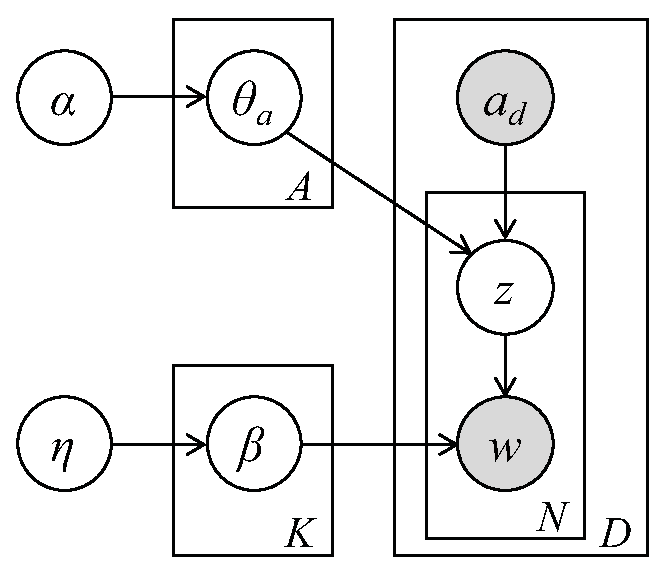
\includegraphics[width=0.3\textwidth]{TATM2.eps}
    \caption{TATM2 in plate notation}
    \label{fig:TATM2}
\end{figure}

The model is shown in Figure \ref{fig:TATM2}. The generative process is as follows:

\begin{enumerate}
	\item For $k \in {1, \ldots, K}$:
	\begin{itemize}
		\item Draw topic $\beta_k \sim \text{Dir}_V(\eta)$.
	\end{itemize}
	\item For $a \in {1, \ldots, A}$:
	\begin{itemize}
		\item Draw author's topic proportions $\theta_a \sim \text{Dir}_K(\alpha)$.
	\end{itemize}
  \item For each document (tweet) $d \in {1, \ldots, D}$:
	\begin{itemize}
		\item For each word $w \in {1, \ldots, N}$:
		\begin{itemize}
			\item Draw topic assignment $z_{d,n} \sim \text{Mult}_K(\theta_a)$.
			\item Draw word $w_{d,n} \sim \text{Mult}_V(\beta_{z_{d,n}})$.
		\end{itemize}
	\end{itemize}
\end{enumerate}


Given the hyperparameters $\alpha$ and $\eta$, the joint distribution of topics $\beta$, author-topic mixture $\theta$, topic assignments $\mathbf{z}$ and words $\mathbf{w}$ is given by:

\begin{equation}
p(\theta,\beta,\mathbf{z},\mathbf{w}|\alpha,\eta) = p(\theta|\alpha) p(\beta|\eta) \prod_{n=1}^{N}{p(z_n|\theta)p(w_n|z_n,\beta_{z_{d,n}})}
\end{equation}


\subsection{Complete conditionals}

First, we denote $\theta_a$ to be the topic proportions of the author $a$ of document $d$, i.e. $\theta_a = \theta_{a_d}$.

\textbf{Local hidden variables.} The complete conditional of the topic assignment $z_{d,n}$ is a multinomial,

\begin{equation}
p(z_{d,n} = k | \theta_a, \beta, w_{d,n}) \propto \exp \{ \log \theta_{a,k} + \log \beta_{k,w_{d,n}} \}
\end{equation}

\textbf{Global hidden variables.} In contrast with standard LDA, the topic proportions are now a global hidden variable.
The complete conditional of the author-topic proportions is a posterior Dirichlet,

\begin{equation}
p(\theta_a | \beta, z_{d}) \propto \text{Dir} ( \alpha + \sum_{d \in D_a}{\sum_{n=1}^{N}{z^k_{d,n}}}),
\end{equation}

\noindent where $D_a$ is the set of documents whose author is $a$.

Finally, the complete conditional for the topic $\beta_k$ is also a posterior Dirichlet,

\begin{equation}
p(\beta_k | \mathbf{z}, \mathbf{w}) \propto \text{Dir} ( \eta + \sum_{d=1}^{D}{\sum_{n=1}^{N}{z^k_{d,n}w_{d,n}}})
\end{equation}



\subsection{Variational parameters for batch variational inference}

The variational parameters are:
\begin{itemize}
	\item Global per-topic Dirichlets $\lambda_{1:K}$
	\item Global per-author Dirichlets $\gamma_{1:A}$
	\item Local per-word multinomials $\phi_{1:D,1:N}$
\end{itemize}

Each update of the local variables is defined as
\begin{equation}
\phi_{d,n} \propto \exp \{ \Psi(\gamma_a) + \Psi(\lambda_{.,w_{d,n}}) - \Psi(\sum_{v}{\lambda_{.,w_{d,n}}}) \}
\end{equation}

Each update of the global variational Dirichlets is defined as
\begin{equation}
\gamma_a = \alpha + \sum_{d \in D_a}{\sum_{n=1}^{N}{\phi_{d,n}}}
\end{equation}

\begin{equation}
\lambda_k = \eta + \sum_{d=1}^{D_a}{\sum_{n=1}^{N}{\phi^k_{d,n}w_{d,n}}}
\end{equation}



\subsection{Stochastic variational inference}

Each update of the local variables is defined as
\begin{equation}
\phi^k_{d,n} \propto \exp \{ \mathbb{E}[\log \theta_{a,k}] + \mathbb{E}[\log \beta_{k,w_{d,n}}] \}
\end{equation}

During the updates of local variables, we utilize an intermediate local variable $\hat{\gamma}_d$, which serves as an indicator of convergence of $\phi_{d}$ during the inner loop of the E-step. Specifically,
\begin{equation}
\hat{\gamma}_d = \sum_{n=1}^{N}{\phi_{d,n}}
\end{equation}


After fitting the local variables, we set the intermediate topics as
\begin{equation}
\hat{\lambda}_k = \eta + D \sum_{d=1}^{D_a}{\sum_{n=1}^{N}{\phi^k_{d,n}w_{d,n}}}
\end{equation}

Finally, the global topics and the global per-author distributions are updated as
\begin{equation}
\lambda^{t+1}_k = (1 - \rho_t) \lambda^{t} + \rho_t \hat{\lambda}_k
\end{equation}

\begin{equation}
\gamma^{t+1}_a = \gamma^{t}_a + \hat{\gamma}_d
\end{equation}



\end{document}
\section{Tweet Author-Topic Model (with per-tweet topics)}
\begin{figure}[h]
\centering
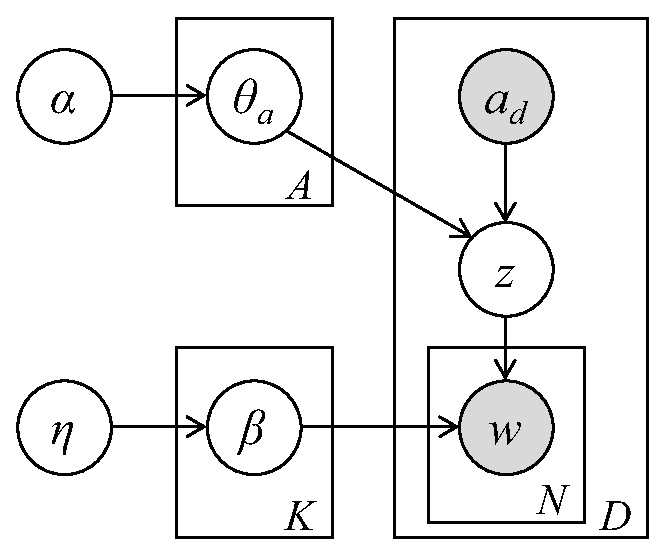
\includegraphics[width=0.3\linewidth]{TATM1}
\caption{Twitter Author-Topic Model with per-tweet topics.}
\label{fig:TATM1}
\end{figure}
This model is shown in figure \ref{fig:TATM1}. The only difference is we now assume a tweet has only one topic assignment, i. e. there is only one hidden variable $z$ per tweet or document. Our corresponding algorithm is shown in Algorithm \ref{alg:stoch_tatm1}. As we have only one local hidden variable per document we can't iteratively optimize it as it is done in the case of online LDA in \cite{Hoffman12}, where there is each document also has a hidden topic. We compute the sufficient statistics $\phi_{d,n}^k$ and then choose the topic $k^*$ which best explains the words in the current document. We then create an intermediate topic distribution for this author $\hat\gamma_a$ consisting of the virtual counts $\alpha$ and the observed counts $N$ in topic $k^*$. We then use this intermediate topic distribution $\hat\gamma_a$ to update author $a$'s topic distribution.
\begin{algorithm}[tb]
\caption{Stochastic variational inference for TATM1}
\label{alg:stoch_tatm1}
\begin{algorithmic}[1]
	\STATE Initialize $\lambda^{(0)}$ randomly.
	\STATE Initialize $\gamma^{(0)} = \alpha$.
	\REPEAT
		\STATE Sample a document $d$ from the data set.
	%\STATE Initialize intermediate local topic proportion $\hat{\gamma}_d = \theta_{a}$.
		%\REPEAT
		\FOR {$k \in \{ 1, \ldots, K \}$}
			\STATE Set $\displaystyle \phi^k_{d} \propto \exp{ \{ \mathbb{E}[\log \theta_{a,k}} ]\} \sum_{n=1}^{N}  \exp \{ \mathbb{E}[\log \beta_{k,w_{d,n}}] \}$.
		\ENDFOR
		\STATE Set intermediate topic $\hat{\lambda}_k = \eta +D \phi_d^k \sum_{n=1}^{N}{w_{d,n}}$.
	%\UNTIL{$\hat{\gamma}_d$ converges}
		%\STATE Set intermediate topics $\hat{\lambda} = \eta + D \sum_{n=1}^{N}{\phi_{d,n}w_{d,n}}$.
		\STATE Set global topics $\lambda^{(t+1)} = (1 - \rho_t) \lambda^{(t)} + \rho_t \hat{\lambda}$.
		%\STATE Set global per-author topic proportions $\gamma^{(t+1)}_a = \gamma^{(t)}_a + \hat{\gamma}_d$.
		\STATE Set intermediate author topic proportion $\hat{\gamma}_a = \alpha +  N \phi_d$.
		\STATE Set global author topic proportions $\gamma_a^{(t+1)} = (1 - \rho_t) \gamma_a^{(t)} + \rho_t \hat{\gamma}_a$.
	\UNTIL{forever}
\end{algorithmic}
\end{algorithm}
\section{Experiments}
%
\subsection{Methodology}\label{sec:methodology}
%
\subsubsection{Data}\label{sec:data}
%
We use our own dataset consisting of 328,428 tweets by 1,876 different users. In brief, it was obtained by selecting a set of 50 popular \textit{core users} from 5 randomly selected categories and crawling Twitter users' posts in a breadth-first search manner by traversing the followee graph. The data was then pre-processed with stemming and stop-word removal.
%
\subsubsection{Software}\label{sec:code}
%
As a base for our code we use an open source online LDA variational bayes package made available by Matt Hoffman\footnote{\url{http://www.cs.princeton.edu/~blei/downloads/onlineldavb.tar}}. We adapted it to incorporate our models and used the included online LDA methods as a benchmark against our models.
%
\subsection{Topic Model Evaluation}
\subsubsection{Perplexity Evaluation}
%
%We use the standard metric perplexity \cite{RefWorks:138} to evaluate the topic model's capability of predicting unseen data. 
%
%We use the data from 286 users for training. As the heldout testing data, we use the remaining 20 users' data. 
%
After training the model on the training dataset, we compute the perplexity of heldout data to evaluate the models.
%
A lower perplexity score indicates better generalization performance of the model. The baseline we choose is Latent Dirichlet Allocation (LDA). Specifically, we calculate perplexity of heldout data by the following equation:
%
\vspace{-1mm}
%
\begin{equation}
	\textrm{Perplexity}({D}_{test}|\mathcal{M})=\exp(-\frac{{\sum}_{d\in D_{test}} \log p(\overrightarrow{w}_{d}|\mathcal{M})}{{\sum}_{d\in D_{test}} N_d}),
\end{equation}
%
\noindent where $\mathcal{M}$ is the model learned from the training dataset, $\overrightarrow{w}_{d}$ is the word vector for document $d$ and $N_d$ is the number of words in $d$.
%
\subsubsection{Topic Distinctiveness}
%
%To evaluate the distinctiveness of the discovered topics, we use the Kullback-Leibler divergence \cite{KL}.
%
KL-divergence is a standard metric to evaluate the distance between two distributions, defined as $D_{KL}(p||q) = \sum{p(i) \cdot log_2(\frac{p(i)}{q(i)})}$. In our work, we calculate the average KL-divergence of each pair of topics. The higher the average KL-divergence, the more distinct the discovered topics are.
%
\subsection{Results} \label{sec:results}
%
\begin{figure}[ht]
\advance\leftskip-4cm
\centering
\subfigure[$\kappa_\textrm{LDA}$]{
	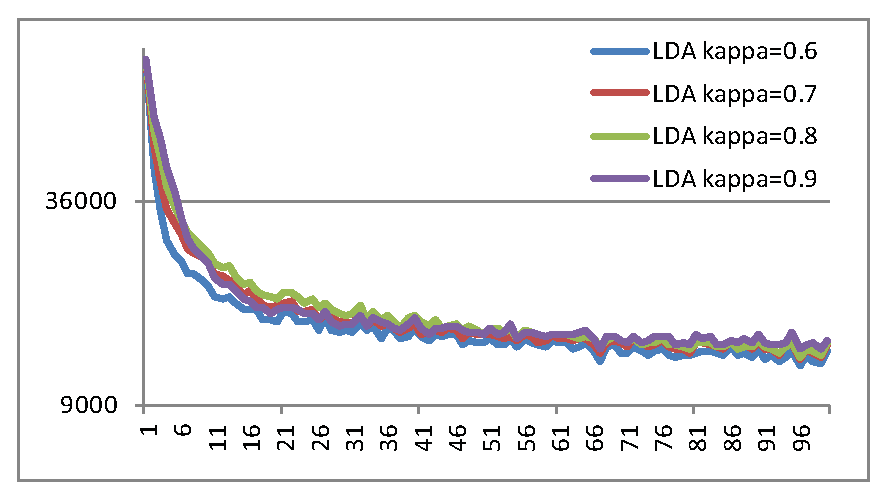
\includegraphics[width=\figwidth,height=\figheight]{kappa_lda}
	\label{fig:kappa_lda}
}
\subfigure[$\kappa_\textrm{TATM1}$]{
	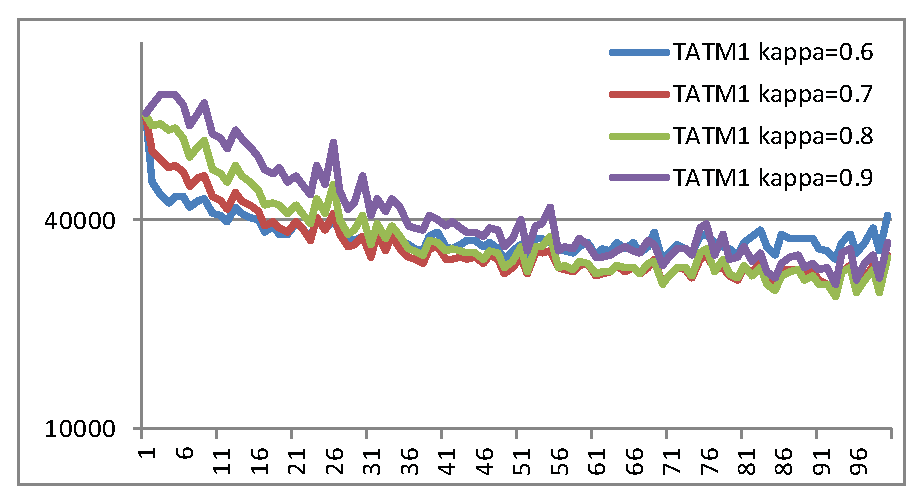
\includegraphics[width=\figwidth,height=\figheight]{kappa_tatm1}
	\label{fig:kappa_tatm1}
}
\subfigure[$\kappa_\textrm{TATM2}$]{
	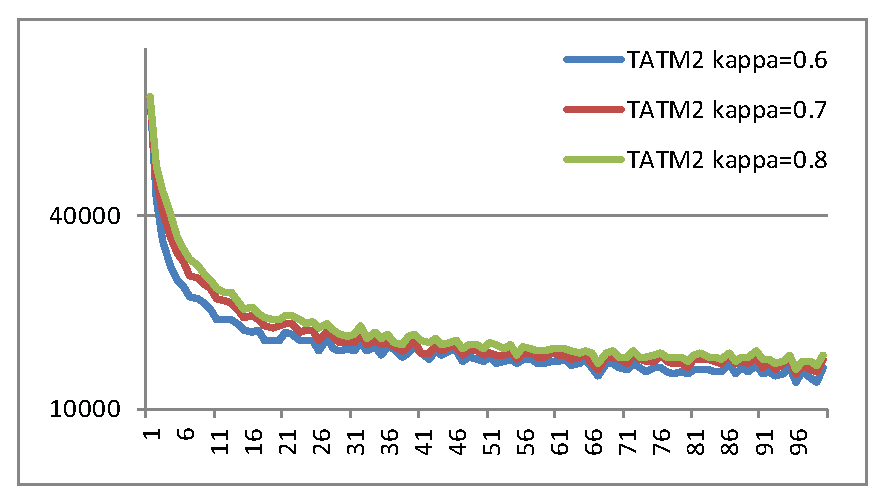
\includegraphics[width=\figwidth,height=\figheight]{kappa_tatm2}
	\label{fig:kappa_tatm2}
}
\subfigure[$\kappa_\textrm{LDA}$]{
	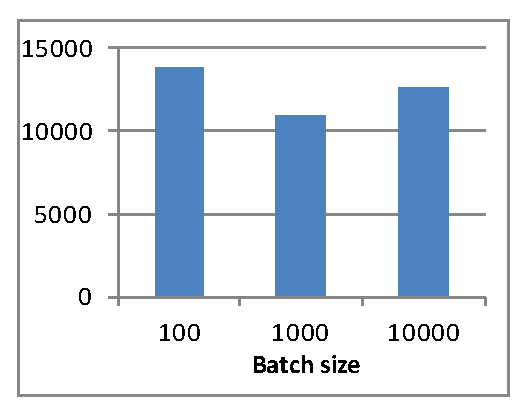
\includegraphics[width=\figwidth,height=\figheight]{batch_lda}
	\label{fig:batch_lda}
}
\subfigure[$\kappa_\textrm{TATM1}$]{
	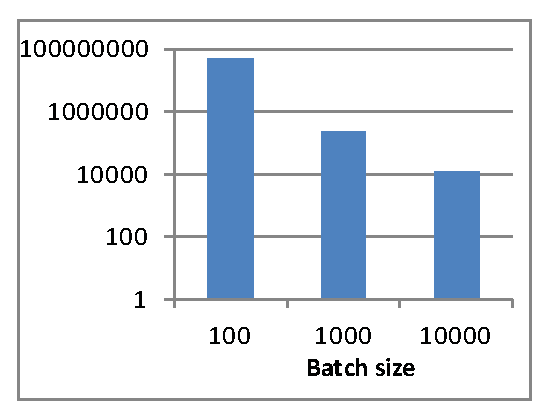
\includegraphics[width=\figwidth,height=\figheight]{batch_tatm1}
	\label{fig:batch_tatm1}
}
\subfigure[$\kappa_\textrm{TATM2}$]{
	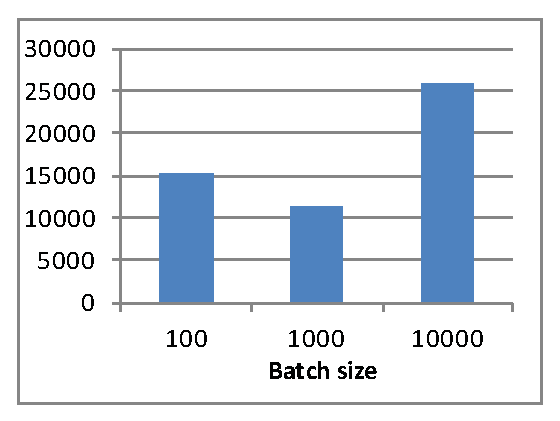
\includegraphics[width=\figwidth,height=\figheight]{batch_tatm2}
	\label{fig:batch_tatm2}
}
\subfigure[$\tau_\textrm{LDA}$]{
	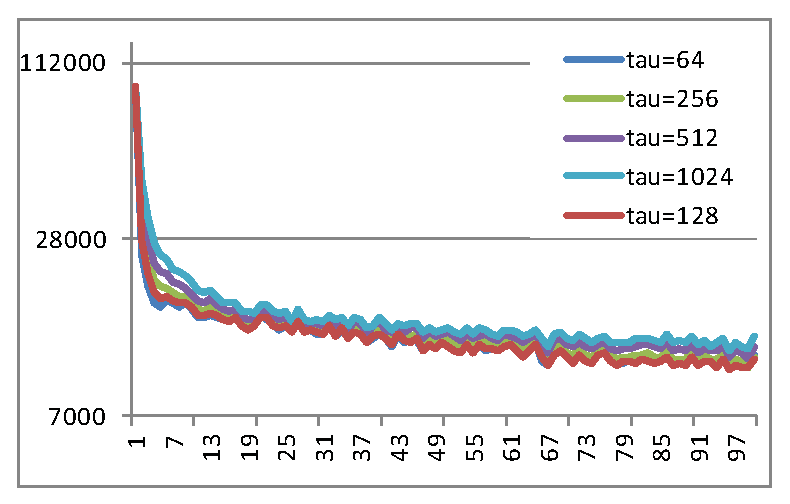
\includegraphics[width=\figwidth,height=\figheight]{tau_lda}
	\label{fig:tau_lda}
}
\caption[Optional caption for list of figures]{Comparison of LDA, TATM1 and TATM2. The vertical axis shows the perplexity and the horizontal axis time $t$ in number of mini-batches processed unless otherwise specified.}
\label{fig:evaluation}
\end{figure}
%
We compare the perplexity for the there models and different values of the \textit{forgetting rate} $\kappa$, the delay $\tau$ and the size of the mini-batches $D$ in figure \ref{fig:evaluation}. LDA and TATM2 are rather insensitive towards the choice of $\kappa$, while for TATM1 lower values of $\kappa$ lead to better results. Overall LDA and TATM2 perform similarly while the results obtained with TATM1 show a perplexity about three times larger after 100 mini-batches have been processed. In general choosing lower values of $\kappa$ increases the initial rate of convergence.

Figures \ref{fig:batch_lda}, \ref{fig:batch_tatm1} and \ref{fig:batch_tatm2} show the final perplexity for batch sizes of 100, 1000 and 10,000. LDA generally delivers the best results and is the least sensitive to choice of batch size. An intermediate batch size of 1000 is the best choice for LDA. TATM1 performs very poorly with the smaller batch sizes but the performance of TATM2 is worst with the larger batch size.

Figure \ref{fig:tau_lda} shows the perplexity for various values of the delay $\tau$ for LDA. The delay down-weighs earlier mini batches. Larger values of $\tau$ lead to both faster convergence and better final results. For TATM1 and TATM2 the dependence is similar and the figures have been omitted.
%
\begin{table}[h]
\centering
\begin{tabular}{l||r|r|r|r|r}
K	&5 &	10&	50	&100&	200 \\ \hline \hline 
LDA	&5503&	6408&	10013 &10816	&11878\\ \hline
TATM1&	9006	&12484&	20039&	102460&	3856537 \\ \hline
TATM2&	5866	&7582&	9922&	10711& 11976 \\
\end{tabular}
\caption{Final perplexity comparison for various values of the number of topics $K$.}
\label{tab:perplexity}
\end{table}
%
\begin{table}[h]
\centering
\begin{tabular}{l||r|r|r|r|r}
K	&5 &	10&	50	&100&	200 \\ \hline \hline 
LDA	&11204897	&7252903	&2174350	&1163910 &615135  \\ \hline
TATM1	&216851 &158863	&10335	&6457	&3923 \\ \hline
TATM2	&11816694	&7907283&	2170469	&1157004 &613705  \\
\end{tabular}
\caption{Final KL divergence comparison for various values of the number of topics $K$.}
\label{tab:kl}
\end{table}
%
\section{Conclusion}
We have set out with the goal of creating a model to determine the interests of twitter users based on their tweets. Due to twitter specific properties and for reasons of scalability we require an online learning algorithm. Based on magnificent work by Blei, Hoffman and others in the field of topic modelling we were able to create two similar models that solved the task at hand reasonably well.

Finally we note that this was arguably too challenging a project to complete in one semester without much prior knowledge about the topic. As a result there is lot left to be done. Ideally we would use a hierarchical Dirichlet Process such that the model can discover the number of topics and create new ones once when necessary.
\printbibliography
\end{document}
